\documentclass{tmr}

\usepackage{mflogo}

%include lhs2TeX.fmt
%include lhs2TeX.sty
%include polycode.fmt

\title{High Performance Haskell with MPI}
\author{Bernie Pope\email{bjpope@unimelb.edu.au}}
\author{Dmitry Astapov\email{dastapov@gmail.com}}

\newcommand{\Todo}[1]{{\textbf{Todo: #1}}}

\begin{document}

\begin{introduction} 
What is MPI, what is haskell-mpi, how can you use it for writing multi-node programs in Haskell or interoperate with other languages
\end{introduction}

\section{Distributed-memory parallelism and MPI}

The World's largest supercomputers now feature hundreds of thousands of CPU cores, and mega-core machines
are just around the corner.\footnote{As one example, the Lawrence Livermore National Laboratory
is preparing to install Sequoia, a 1.6 million core IBM BlueGene/Q (\url{https://asc.llnl.gov/computing_resources/sequoia/}).} There are many technical
challenges to building such behemoths, not the least of which is
the CPU-to-memory bottleneck. Shared memory parallel computers --- which now dominate consumer-grade
systems --- provide the convenient abstraction that every processor has equivalent access to all memory,
even though the underlying connections between processors and memory are typically non-uniform.
Unfortunately (and unsurprisingly) it is difficult to scale this abstraction in a
cost-effective way beyond a few thousand cores. A quick glance at the Top 500 list of supercomputers reveals
no significant large-scale shared-memory systems in recent years.\footnote{\url{http://www.top500.org/}}
Instead we see that practically all the listed supercomputers are based on
distributed-memory parallelism. These machines are built from many independent computers (called nodes),
each with their own processors, memory and operating system, interconnected by one or more high-speed networks.
The nodes themselves are often smaller multi-core shared-memory computers, nevertheless
the macro architecture is distributed.

Distributed-memory parallelism does not really solve the CPU-to-memory bottleneck (over the whole machine),
after all, sharing data between nodes over a network is a relatively costly operation.
Instead it forces programmers to
address the non-uniformity head on, which typically means adopting an explicitly distributed style of
parallel programming, and often requires new algorithms to be devised.

The Message Passing Interface (MPI) is a ``message-passing library interface specification''
for writing distributed-parallel programs~\cite{mpi-report}. Various realizations of the
specification are provided by software libraries, some of which are open source
(such as OpenMPI\footnote{\url{http://www.open-mpi.org/}} and MPICH\footnote{\url{http://www.mcs.anl.gov/research/projects/mpich2/}}), and some of which are proprietary.
As the name suggests, MPI is firmly rooted in the paradigm of message passing.
An MPI application consists of numerous independent computing processes (or tasks)
which collaborate by sending messages amongst themselves.
The underlying communication protocols are programming language agnostic, but standard APIs are
defined for Fortran, C and C++. Bindings in other languages, such as Haskell-MPI,
are typically based on foreign interfaces to the C API.

Haskell-MPI provides a fairly modest wrapping of MPI, and is guided by two objectives:
\begin{enumerate}
 \item Convenience: for a small cost, it should be easy to send arbitrary (serialisable)
data structures as messages.
 \item Performance: low overhead communications should be possible,
particularly for array-like data structures.
\end{enumerate}
It is difficult to satisfy both objectives in one implementation, so Haskell-MPI provides two interfaces.
The first is simple to use (more automated) but potentially slower (more data copying), the second
is more cumbersome to use (less automated) but potentially faster (less data copying).

This article aims give you a taste of distributed parallel programming with Haskell-MPI, enough to
whet your appetite, without getting too bogged down in details. Those who find themselves hungry for
more can consult the haddock pages for a more substantial course and check out examples in the package sources.

We begin by introducing the technique of computing definite integrals by the trapezoid method.
This lends itself to an easy-to-parallelise algorithm which will serve as the
basis of programming examples in the following sections. We take a simple sequential implementation
of the algorithm, and morph it into two different parallel implementations.
The first uses shared-memory and threads, and the second uses distributed-memory and Haskell-MPI.
To see how well we fare against the conventional school, we also provide an MPI implementation in C.
We then evaluate the performance of each version on a non-trivial problem instance and compare the results.
We conclude by discussing some of the more interesting features of Haskell-MPI that were not covered in
previous sections, and show how Haskell-MPI and C-MPI can coexist in a single parallel computation.

%\section{Very short intro to MPI and haskell-mpi and outlining the motivation}
%What is MPI? If you ever tried to make processes running on separate
%computers talk to each other, chances are that you already came across
%the MPI or invented parts of it. 

%Even though MPI has been standartized only aroung 1995\footnote{Full
%  formal definition of protocol, its semantics and reference
%  implementation could be found in \cite{mpi-report}}, it has become
%de-facto standart in programming on architecures with distributed
%memory (``clusters'' or ``parallel computers''). It tries to prove a
%language-independent communications means that would allow users to
%pass around ``messages'' (hence the name, ``Message Passing
%Interface''). We have it on a good authority that MPI is still widely
%used today, even though there are numerous alternatives for
%inter-process communication. This article would focus on haskell-mpi,
%not trying to provide any sort of comparison with possible
%alternatives, as authors believe that any choice like this should
%ultimately be made in context of the specific task at hand.

%So what is, then, haskell-mpi? It is a package of low- and high-level bindings
%to C MPI library that allows Haskell programmers to call upon the
%powers of MPI with ease. 

%What would be the most (stereo)typical use case for haskell-mpi?
%Suppose that you have a task which easily lends itself to subdivision
%into a number of independent subtasks. In this day and age, when
%having multiple networked computers in vicinity is more of a rule than
%an exception, it is only natural to try and execute all the subtasks
%on different machines in parallel and then combine their results.

\section{Computing definite integrals with trapezoids}

\begin{figure*}[t]
\centering
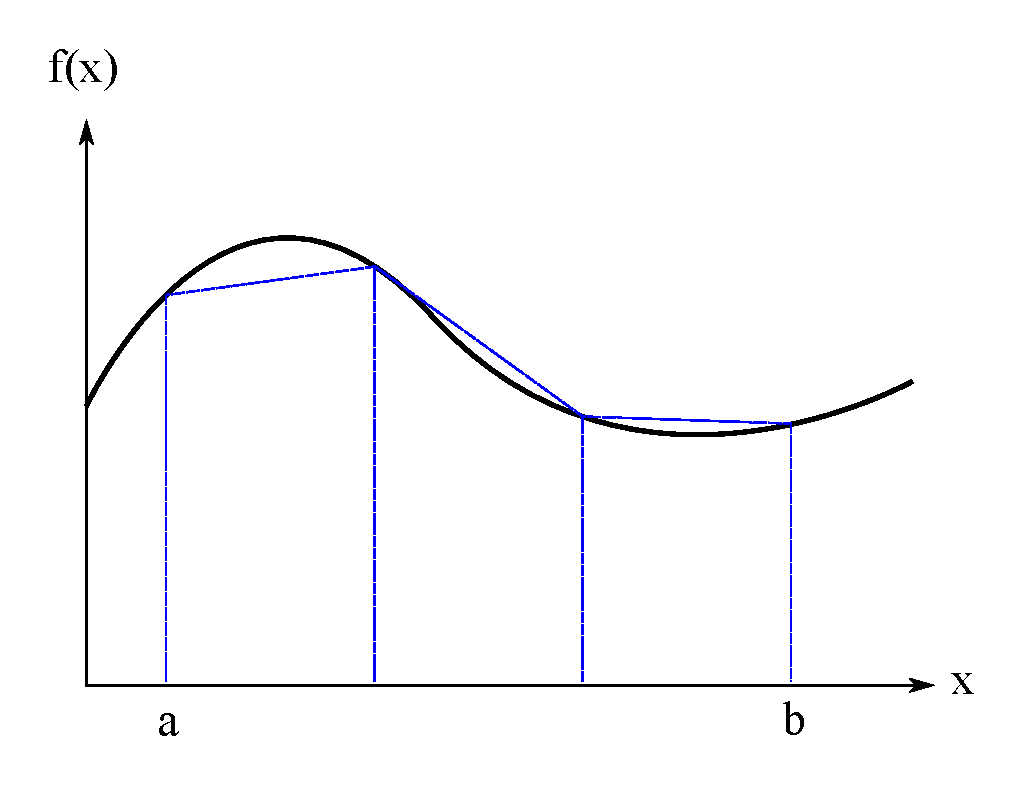
\includegraphics[width=8cm]{integral_diag.pdf}
\caption{Approximating $\int_{x=a}^{b} f(x)$ by summing the area of three trapezoids.
\label{trapezoidfig}}
\end{figure*}

We now consider the problem of computing definite integrals
using the trapezoid method. The algorithm is naturally data parallel, and is a common
introductory example in parallel programming tutorials. Our presentation is inspired by
Pacheco's textbook on MPI~\cite{Pacheco}.
We can approximate integrals by summing the area of a consecutive
trapezoids lying under a function within a given interval, as illustrated in
Figure~\ref{trapezoidfig}. A single trapezoid spanning the interval
$[x_0,x_1]$ has area:
\begin{equation*}
\frac{(x_1 - x_0)(f(x_0) + f(x_1))}{2}
\end{equation*}
Extending this to $n$ equally spaced sub-intervals $[x_0,x_1,\ldots,x_n]$ we arrive at the formula:
\begin{equation*}
\begin{split}
\int_{x=a}^{b} f(x)\ \approx\ &\ \frac{h}{2} \sum_{i=1}^n f(x_{i-1}) + f(x_i) \\[3mm]
                     \approx\ &\ h \left(\frac{f(x_0) + f(x_n)}{2} + f(x_1) + \ldots + f(x_{n-1})\right) \\[3mm]
                     &\ x_0 = a,\ x_n = b,\ h = (b - a)/n\\
                     &\ \forall i \in \{0 \ldots n-1\},\ x_{i+1} - x_{i} = h
\end{split}
\end{equation*}
Listing \ref{Trapezoid} provides a sequential implementation of the trapezoid method in Haskell, with
the integrated function defined to be $f(x) = 4 / (1 + x^2)$.

% ./code/Trapezoid.hs
\begin{listing}
\begin{Verbatim}
module Trapezoid (trapezoid, f) where

trapezoid :: (Double -> Double)  -- Function to integrate
             -> Double -> Double -- integration bounds
             -> Int              -- number trapezoids
             -> Double           -- width of a trapezoid
             -> Double
trapezoid f a b n h =
  h * sum (endPoints:internals)
  where
  endPoints = (f a + f b) / 2
  internals = map f $ take (n - 1) $ iterate (+h) (a + h)

f :: Double -> Double
f x = 4 / (1 + x * x)
\end{Verbatim}
\caption{Calculating definite integrals using the trapzoid method. \label{Trapezoid}}
\end{listing}

Using this module, we could write a simple program that would take
\verb|a|, \verb|b| and \verb|n| from the command line and show results
of integration (see listing \ref{single-threaded}).

\begin{listing}
\begin{Verbatim}
module Main where

import System (getArgs)
import Trapezoid

main :: IO ()
main = do
  aStr:bStr:nStr:_ <- getArgs
  let [a,b] = map read [aStr,bStr]
      n = read nStr
      h = (b - a) / fromIntegral n
      integral = trapezoid f a b n h
  print integral 
\end{Verbatim}
\caption{Sequential program for calculating definite integrals. \label{single-threaded}}
\end{listing}


% I took this out because it might be misleading about what the error means.
%We can use this program to approximate $\pi$
%by choosing $[0,1]$ as the interval for integration. The following table shows, for increasing interval sizes,
%the error of the program's output compared to the
%value of |pi :: Double| from the Haskell Prelude.
%
%\begin{center}
%\begin{tabular}{|l|l|l|}
%\hline
%intervals & error \\ \hline\hline
%$10^0$ & $1.4 \times 10^{-1}$ \\ \hline
%$10^1$ & $1.7 \times 10^{-3}$ \\ \hline
%$10^2$ & $1.7 \times 10^{-5}$ \\ \hline
%$10^3$ & $1.7 \times 10^{-7}$ \\ \hline
%$10^4$ & $1.7 \times 10^{-9}$ \\ \hline
%$10^5$ & $1.6 \times 10^{-11}$ \\ \hline
%$10^6$ & $-1.3 \times 10^{-12}$ \\ \hline
%\end{tabular}
%\end{center}


%After splitting interval into arbitrary number of parts you could
%integrate them separately and them sum the results. In fact, very
%simple modification is required to make this code use all available
%cores in single multi-cored machine:
%% ./code/Trapezoid-threads.hs

\section{Parallelization of the trapezoid method on a single machine}

The trapezoid method is a classic data-parallel problem because
the computations on each sub-interval can be computed independently.
For an interval $[a,b]$, $n$ sub-intervals, and $p$ processors, we can parallelize
the algorithm using a simple chunking scheme like so:
\begin{enumerate}
   \item The master processor splits the sub-intervals into chunks of size $s = n/p$.
   \item In parallel, each processor $p_i$ computes the definite intergal on the sub-interval 
         $[a_i, b_i]$, where $h = (b - a)/n$, $a_i = a + i \times s \times h$ and
         $b_i = a_i + s \times h$.
   \item The master processor collects the results for each chunk and sums them up.
\end{enumerate}
Listing~\ref{multi-threaded} shows that it is quite easy to use threads to
parallelize the trapezoid program, thanks to the convenient combinators provided by the
parallel strategies library.

\begin{listing}
\begin{Verbatim}
module Main where

import GHC.Conc
import Control.Parallel.Strategies

import System (getArgs)
import Trapezoid

main :: IO ()
main = do
  let maxThreads = numCapabilities
  aStr:bStr:nStr:_ <- getArgs
  let [a,b] = map read [aStr,bStr]
      n = read nStr
      h = (b - a) / fromIntegral n
      localN = n `div` fromIntegral maxThreads
      chunks = parMap rseq (\threadNo ->
         let localA = a + fromIntegral threadNo * fromIntegral localN * h
             localB = localA + fromIntegral localN * h
             in trapezoid f localA localB localN h) [0..maxThreads-1]
  print (sum chunks)
\end{Verbatim}
\caption{Multi-threaded parallel program for calculating definite integrals using the trapzoid method. \label{multi-threaded}}
\end{listing}

%% ideas for further sections: show how easy it would be to extend this to ``find number of nodes AND number of cores on them, split work according to power of node''

\section{Parallelization on multiple machines using MPI}

\subsection{Point-to-point communications}

We could use the same chunking approach to spread computations over
several machines using MPI. Work would be evenly divided among all
processes participating in the single execution run, and one of them
would be designated ``master'', responsible for collecting results for
each chunks and computing final result. 

In previous example each thread had a simple numeric index, whereas
MPI uses more complex two-level numbering scheme for processes.
Whenever you had to designate sender or receiver of the message, you
have to specify numeric ID of the process group (``communicator'' in
MPI terminology), and unique number of the process within the group.
Each process could participate in the arbitrary number of groups,
which could be created and destroyed at run time. By defailt, all
processes are made members of the single pre-defined communicator
called ``world''.

MPI allows synchronous and asynchronous sending and receiving of
messages, but even in synchronous mode there is no requirement for
messages to be processed in the same order. Instead MPI introduces a
concept of numeric ``tag'' which allows sender and receiver to
distinguish between different messages of the same type.

Beside simple process-to-process message sending and receiving, MPI
provides one-to-many, many-to-one and many-to-many communication
primitives, capturing majority of the typical real-world communication
scenarios.

Listing \ref{mpi-p2p} shows how we could parallelize our task using
point-to-point communication functions.

\begin{listing}
\begin{Verbatim}
module Main where

import Control.Parallel.MPI.Simple
import System (getArgs)
import Trapezoid

main :: IO ()
main = mpi $ do
  numRanks <- commSize commWorld
  rank <- commRank commWorld
  let master = 0 :: Rank
      
  aStr:bStr:nStr:_ <- getArgs
  let [a,b] = map read [aStr,bStr]
      n = read nStr
      h = (b - a) / fromIntegral n
      localN = n `div` fromIntegral numRanks
      localA = a + fromIntegral rank * fromIntegral localN * h
      localB = localA + fromIntegral localN * h
      integral = trapezoid f localA localB localN h
      messageTag = 123 :: Tag
  if rank == master then do 
    rest <- sequence [ recv' commWorld (toRank proc) messageTag 
                     | proc <- [1..numRanks-1] ]
    print (integral + sum rest)
    else send commWorld master messageTag integral
  where
    recv' comm rank tag = do 
      (msg, status) <- recv comm rank tag
      return msg
\end{Verbatim}
\caption{Multi-node parallel program for calculating definite
  integrals, using point-to-point communication. \label{mpi-p2p}}
\end{listing}
%% $

We've chosen number $123$ as a ``tag'' for our messages, and process
with ID (``rank'') of zero is designated to be the ``master''. Master
would execute a sequence of synchronous receive operations to collect
result from the rest of the processes and then add its own piece of
work to compute the total. Messages that arrive to master before he is
ready to receive them would be kept by MPI in internal buffer until
the appropriate receive operation is executed. Status of the receive
operations would be discarded in \verb|recv'| for brevity.

It might seem strange at first that processes do no exchange any
messages to determine how the work would be divided among them. That is
because an established practice in MPI world is to run the same binary
on all computers (``nodes'') participating in the run, to reduce
development and deployment efforts. Therefore, if some run-time
parameters could be deduced solely from process rank plus
some information available to all processes at startup, it would not
require any additional message passing.

This way, programs that use MPI usually features a substantial amount of code,
which, while present in all binaries, is actually executed only in
some of the running copies. While programming with MPI in C, care must
be taken to avoid allocations/computations in processes that would not
actually use the appropriate data, and to avoid referencing/using
uninitialized data. Haskell, with its lazy evaluation and automatic
memory management, allows to significantly reduce amount of mental
energy required to get everything right. If computations are pure,
they simply would not be executed in the processes that don't use
them, without requiring any explicit ``housekeeping'' code.

\subsection{Many-to-one communications}

Use of the point-to-point communications in the previous section leads
to a number of unwanted side-effects. First of all, master process
tries to receive messages from other processes sequentially. It would
not have large effect on our toy example, but in real application with
messages that have significant size (and, therefore, significant
transfer time) it would be much better if we could receive them in
parallel, as soon as they are sent. 

Another problem lies in the fact that master process would not try to
perform its piece of work until after it received messages from all
the other processes. It would be much better if master process would
perform its share of the computations at the same time as other
processes do, instead of spending this time waiting for messages.

To overcome this deficiencies we could switch to asynchronous
(non-blocking) receiving, but this would make our code much more
verbose.

Instead, we would use one of the many-to-one communication operations
provided by MPI, called ``gather''. As before, one of the processes
have to be designated ``master'', which would perform ``gather
receive'', and all the other processes would perform ``gather send''
of the computed results. As you could see in listing \ref{mpi-gather},
this leads to a short and succint implementation.

\begin{listing}
\begin{Verbatim}
module Main where

import Control.Parallel.MPI.Simple
import System (getArgs)
import Trapezoid

main :: IO ()
main = mpi $ do
  numRanks <- commSize commWorld
  rank <- commRank commWorld
  let master = 0 :: Rank
  
  aStr:bStr:nStr:_ <- getArgs
  let [a,b] = map read [aStr,bStr]
      n = read nStr
      h = (b - a) / fromIntegral n
      localN = n `div` fromIntegral numRanks
      localA = a + fromIntegral rank * fromIntegral localN * h
      localB = localA + fromIntegral localN * h
      integral = trapezoid f localA localB localN h
  if rank == 0
     then print . sum =<< gatherRecv commWorld master integral
     else gatherSend commWorld master integral
\end{Verbatim}
\caption{Multi-node parallel program for calculating definite
  integrals, using many-to-one communication. \label{mpi-gather}}
\end{listing}
%% $

It might seem strange to specify rank of the master process in call to
\verb|gatherRecv|. It seems even stranger to pass \verb|integral|
there -- after all, it would be essentially just returned back
immediately as a part of collected results, isn't it? This particular
odditiy is necessary to accomodate the feature of MPI called
``intercommunicators'' where group of processes could pose as master
in one-to-many or many-to-one communications, allowing to speed up
collection and processing of collected results\footnote{This rather
  advanced topic would not be discussed in greated detail here.
  Readers are encouraged to refer to more academic sources on MPI,
  like \cite{2}}.

\section{Peformance comparison}

In order to compile and run our sample integration code, you have to
have \verb|haskell-mpi| package installed\footnote{Please refer to
  \ref{appendix-A}{Appendix A} for installation and running help}. After that,
simple \verb|ghc --make -O2 <file>.hs| should be sufficient to produce
a working MPI-enabled binary.

Even if you don't have several networked computers, you could still
run several processes on the same box, which actually makes sense if
you have multiple CPU cores. OpenMPI would do this by default if you
haven't configured your ``computing network'' topology. Try running
\verb|mpirun -n <N> ./ToDoNameHere ToDoArgsHere|, where \verb|N| is
from 1 up to the number of cores you have.

You should be able to observe almost linear speed up. We were able to
test this code on quite large computing cluster and got the following
numbers\footnote{runtimes from N tries, averaged}:

%\Todo: measurement results here, table and graph. Measure simple version, threaded and MPI against each other

\begin{figure}
\begin{minipage}[b]{0.5\linewidth}\centering
\begin{tabular}{|l|l|l|l|} \hline
method & cores & $n$ & time(s) \\ \hline\hline
single & 1     & $10^7$ & 1.040 \\ \hline\hline
threaded & 1   & $10^7$ & 1.046 \\ \hline
threaded & 2   & $10^7$ & 0.617 \\ \hline
threaded & 4   & $10^7$ & 0.308 \\ \hline
threaded & 8   & $10^7$ & 0.184 \\ \hline\hline
mpi & 1   & $10^7$ & 1.118 \\ \hline
mpi & 2   & $10^7$ & 0.576  \\ \hline
mpi & 4   & $10^7$ & 0.319 \\ \hline
mpi & 8   & $10^7$ & 0.255 \\ \hline
mpi & 16  & $10^7$ & 2.248 \\ \hline
\end{tabular}
\end{minipage}
\hspace{0.5cm}
\begin{minipage}[b]{0.5\linewidth}
\centering
\begin{tabular}{|l|l|l|l|} \hline
method & cores & $n$ & time(s) \\ \hline\hline
single & 1     & $10^9$ & 114.872 \\ \hline\hline
threaded & 1   & $10^9$ & 104.662 \\ \hline
threaded & 2   & $10^9$ & 54.409 \\ \hline
threaded & 4   & $10^9$ & 28.947  \\ \hline
threaded & 8   & $10^9$ & 14.894 \\ \hline\hline
mpi & 1   & $10^9$ & 107.900 \\ \hline
mpi & 2   & $10^9$ & 53.602  \\ \hline
mpi & 4   & $10^9$ & 26.932 \\ \hline
mpi & 8   & $10^9$ & 13.571 \\ \hline
mpi & 16  & $10^9$ & 8.260 \\ \hline
mpi & 32 & $10^9$ & 5.332 \\ \hline
mpi & 64   & $10^9$ & 4.105 \\ \hline
mpi & 128   & $10^9$ & 3.542 \\ \hline
mpi & 256 & $10^9$ & 3.602 \\ \hline
\end{tabular}
\end{minipage}
\vspace{3mm}
\caption{Timing figures for Haskell implementations. \label{TiminigTable}}
%\end{figure}
\end{figure}

\begin{figure}
\begin{center}
\begin{tabular}{|l|l|l|l|} \hline
method & cores & $n$ & time(s) \\ \hline\hline
C-mpi & 1   & $10^9$ & 53.570 \\ \hline
C-mpi & 2   & $10^9$ & 23.664  \\ \hline
C-mpi & 4   & $10^9$ & 12.500 \\ \hline
C-mpi & 8   & $10^9$ & 6.656 \\ \hline
C-mpi & 16  & $10^9$ & 4.142 \\ \hline
C-mpi & 32 & $10^9$ & 3.360 \\ \hline
C-mpi & 64   & $10^9$ & 3.037 \\ \hline
C-mpi & 128   & $10^9$ & 2.861 \\ \hline
C-mpi & 256 & $10^9$ & 2.934 \\ \hline
\end{tabular}
\end{center}
\caption{Timing figures for parallel C implementation using MPI.\label{CTiminigTable}}
%\end{figure}
\end{figure}


As you can see (describe something less obvious that could be derived
from the graph, for example that for large N computation takes less
time than transmission of the results).

\section{Fast API vs Simple API}

Haskell-mpi provides two different APIs suitable for different kinds
of data. Control.Parallel.MPI.Simple, which we used in our examples so
far, allows you to send just about any Haskell type over the wire, as
long as it is an instance of typeclass \verb|Serialize|. This
typeclass is defined in the package \verb|cereal|, which provides
instances for many popular Haskell types. It is expected that user
would write instances for user-defined types themselves, but
fortunately they are quite trivial.

To illustrate that, one of the authors took GitHub project McPhd,
which uses Haskell to simulate particles (\Todo: fix the desc,
copypaste from haskell para report here), and added support for
parallel execution of the simulation using MPI. GitHub patch ... shows
all the changes that were necessary to make this happen.


\section{Interacting with C}
You could use it to combine haskell and C code. Here is how: (separate sub-section on this?)

\begin{Verbatim}
#include <mpi.h>
#include <stdio.h>
#include <stdlib.h>
#include <math.h>

double f(double);
double trapezoid(double, double, int, double);

int main(int argc, char **argv) {
   double a, b, h, local_a, local_b, integral, sum = 0;
   double *results = NULL;
   int n, local_n, rank, num_ranks;

   MPI_Init(&argc, &argv);
   MPI_Comm_size(MPI_COMM_WORLD, &num_ranks);
   MPI_Comm_rank(MPI_COMM_WORLD, &rank);

   a = atof(argv[1]);
   b = atof(argv[2]);
   n = atoi(argv[3]);

   h = (b - a) / n;
   local_n = n / num_ranks;
   local_a = a + rank * local_n * h;
   local_b = local_a + local_n * h;
   integral = trapezoid(local_a, local_b, local_n, h);

   if (rank == 0) {
      results = (double *) malloc(num_ranks * sizeof(double));
   }

   MPI_Gather(&integral, 1, MPI_DOUBLE, results, 1, MPI_DOUBLE, 0, MPI_COMM_WORLD);

   if (rank == 0) {
      for (int i = 0; i < num_ranks; i++) {
         sum += results[i];
      }
      printf("%lf\n", sum);
   }
   MPI_Finalize();
}

double trapezoid(double a, double b, int n, double h) {
   double result;
   double x = a;
   result = (f(a) + f(b)) / 2.0;
   for (int i = 1; i < n; i++) {
      x = x + h;
      result += f(x);
   }
   return result * h;
}

double f(double x) {
   return 4.0 / (1 + x * x);
}
\end{Verbatim}


Or you can you is to implement less trivial communication patterns (allreduce example or something more complex?)


\section{Conclusion, further reading, next steps, ...}

\Todo mention somewhere bundled example and tests that could provide inspiration :)

Full \verb|haskell-mpi| sources\footnote{github, cabal source
  haskell-mpi} also contain a comprehensive testsuite and a set of
examples, which demonstrate the use of all of the supported functions.

\Todo mention Well-Typed

\section{Appendix A: Installation and tested MPI implementations}
\label{appendix-A}
We tested the code on MPICH 1.2.x and 1.4.x, OpenMPI x.y.z. Amount of implementation-specific code is minimal and there is a good chance that all the other MPI implementations would be supported out of the box.

To install, try ``cabal install haskell-mpi''. If that fails to find MPI include/library files in system-wide directories, try ...
\Todo provide installation cmdline

\bibliography{haskell-mpi}

\end{document}
